\documentclass[12pt]{scrartcl}
\usepackage{azzam}


\title{Kombinatorika + Bonus}

\begin{document}
\section{Kombinatorika}
\begin{enumerate}
    \item Misalkan Michie mempunyai 3 buah celana dan 4 buah baju. Berapa banyak cara Michie memilih celana dan baju yang akan dipakai ?

    \item Berapa banyak cara menyusun huruf-huruf R, A, J, I, N jika 
    \begin{enumerate}
        \item huruf pertama dimulai dari huruf hidup (vokal) 
        \item huruf pertama dimulai dari huruf mati (konsonan) 
    \end{enumerate}

    \item Sembilan orang siswa akan duduk pada 5 kursi sejajar. Ada berapa cara susunan mereka ? 
    
    \item Denny akan membentuk bilangan genap 3 angka yang angka-angkanya diambil dari 2, 3, 4, 5, 6, 7, 8. Berapa banyak bilangan yang dapat dibentuk jika : 
    \begin{enumerate}
        \item angka-angkanya boleh berulang 
        \item angka-angkanya tidak boleh berulang
    \end{enumerate}

    \item (OSK 2003) Ada berapa banyak bilangan 4-angka (digit) yang semua angkanya genap dan bukan merupakan kelipatan 2003 ?

    \item Sekumpulan orang duduk mengelilingi sebuah meja bundar. Diketahui ada 7 wanita dimana di sebelah kanan setiap wanita tersebut adalah wanita dan ada 12 wanita yang di sebelah kanan setiap wanita tersebut adalah pria. Diketahui pula bahwa 3 dari 4 pria di sebelah kanannya adalah wanita. Berapa orang yang duduk mengelilingi meja tersebut?

    \item (OSK 2013) Enam orang siswa akan duduk pada tiga meja bundar, dimana setiap meja akan diduduki oleh minimal satu siswa. Banyaknya cara untuk melakukan hal tersebut adalah \ldots

    \item (OSK 2015) Suatu sekolah mempunyai lima kelompok belajar siswa kelas 11. Kelompok-kelompok belajar itu berturut-turut mengirimkan 2, 2, 2, 3, dan 3 siswa untuk suatu pertemuan. Mereka akan duduk melingkar sehingga setiap siswa memiliki paling sedikit satu teman dari kelompok belajar yang sama yang duduk di sampingnya. Banyaknya cara melakukan hal tersebut adalah \ldots\\
    (Dua cara mereka duduk melingkar dianggap sama jika salah satu cara dapat diperoleh dari cara yang lain dengan suatu rotasi)

    \item Berapa banyak orang minimum yang harus hadir di suatu pesta sehingga dipastikan terdapat 3 orang yang lahir di bulan yang sama di pesta itu?

    \item (OSK 2011) Di lemari hanya ada 2 macam kaos kaki yaitu kaos kaki berwarna hitam dan putih. Ali, Budi dan Candra berangkat di malam hari saat mati lampu dan mereka mengambil kaos kaki secara acak di dalam lemari dalam kegelapan. Berapa kaos kaki minimal harus mereka ambil untuk memastikan bahwa akan ada tiga pasang kaos kaki yang bisa mereka pakai ? (Sepasang kaos kaki harus memiliki warna yang sama).

    \item Misalkan Naruko memilih $k$ buah bilangan dari himpunan $\{1,2,3,\dots,2016\}$ secara acak. Berapakah nilai $k$ terkecil sehingga Naruko pasti bisa mendapatkan setidaknya sepasang bilangan (dari $k$ bilangan itu) yang jika dijumlahkan hasilnya 2017?
    
    \item Suatu malam di rumah WonYoung terjadi pemadaman listrik. Karena WonYoung sangat malas, ia hanya ingin tidur dengan membawa banyak kaus kaki (hobi yang aneh :/). Ia mengambil kaus kaki dari lemari di ruangan yang sangat gelap. Lemari itu berisi 100 buah kaus kaki merah, 80 kaus kaki hijau, 60 kaus kaki biru, dan 40 kaus kaki hitam. WonYoung mengambil banyak kaus kaki tapi tidak bisa tahu warnanya. Berapa banyak kaus kaki paling sedikit yang perlu diambil sehingga dijamin terdapat setidaknya 10 pasang kaus kaki (dengan setiap pasang kaus kaki harus berwarna sama) ?
    
    \item (OSK 2016) Anak laki-laki dan anak perempuan yang berjumlah 48 orang duduk melingkar secara acak. Banyaknya minimum anak perempuan sehingga pasti ada enam anak perempuan yang duduk berdekatan tanpa diselingi anak laki-laki adalah \dots
\end{enumerate}

\section{Camilan Geometri}
\begin{enumerate}[resume]

\item Tentukan nilai $x$ pada diagram berikut:
    \begin{figure}[H]
        \centering
        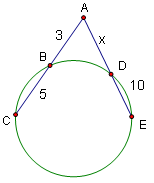
\includegraphics[scale=1]{0Figure/Popprob1.png}
    \end{figure}

\item Tentukan nilai $x$ pada diagram berikut:
    
    \begin{figure}[H]
        \centering
        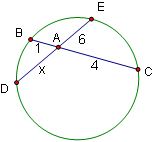
\includegraphics[scale=1]{0Figure/Popprob2.png}
    \end{figure}

\item (ARML) Pada sebuah lingkaran, tali busur $AB$ dan $CD$ berpotongan di $R$. Jika $AR : BR = 1 : 4$ dan $CR : DR = 4 : 9$, tentukan rasio $AB : CD$.
    
    \begin{figure}[H]
        \centering
        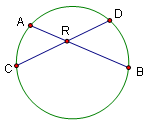
\includegraphics[scale=1]{0Figure/Popprob3.png}
    \end{figure}
    
\item (ARML) Tali busur $AB$ dan $CD$ pada sebuah lingkaran saling tegak lurus dan berpotongan di titik $E$. Diketahui $BE = 16, DE = 4$, dan $AD = 5$, tentukan panjang $CE$.

\item Misalkan $\overline{AB}$ adalah diameter pada lingkaran dengan jari-jari $5\sqrt{2}$. Misalkan $\overline{CD}$ adalah tali busur pada lingkaran tersebut yang memotong $\overline{AB}$ di titik $E$ sedemikian sehingga $BE = 2\sqrt{5}$ dan $\angle AEC = 45^\circ$. Berapakah nilai dari $CE^2 + DE^2$?

\end{enumerate}
\end{document}